\documentclass[conference]{IEEEtran}
\IEEEoverridecommandlockouts
% The preceding line is only needed to identify funding in the first footnote. If that is unneeded, please comment it out.
\usepackage{cite}
\usepackage{amsmath,amssymb,amsfonts}
\usepackage{algorithmic}
\usepackage{graphicx}
\usepackage{textcomp}
\usepackage{xcolor}

\usepackage{epsfig,endnotes}
\usepackage{kotex}
\usepackage{subfig}
\usepackage{comment}
\usepackage[numbers,sort&compress]{natbib}
%\usepackage[breaklinks]{hyperref}
\def\UrlBreaks{\do\/\do-}


\newcommand{\BSK}[1]{\textcolor{red}{#1}}
\newcommand{\EUNJI}[1]{\textcolor{blue}{#1}}
\newcommand{\FOOTBF}[1]{\footnotesize{\bf{#1}}}
\newcommand{\WHERETOGO}[1]{\textcolor{orange}{WHERETOGO: #1}}
\newcommand{\ours}{\texttt{Hexa}-SSD}


\def\BibTeX{{\rm B\kern-.05em{\sc i\kern-.025em b}\kern-.08em
    T\kern-.1667em\lower.7ex\hbox{E}\kern-.125emX}}
\begin{document}

\title{Hexa: Overcoming Capacitance Constraints in SSDs}

% \title{Conference Paper Title*\\
% {\footnotesize \textsuperscript{*}Note: Sub-titles are not captured in Xplore and
% should not be used}
% \thanks{Identify applicable funding agency here. If none, delete this.}
% }

\author{\IEEEauthorblockN{Sanghyun Nam, Seungmin Shin}
\IEEEauthorblockA{%\textit{dept. of AI Convergence} \\
\textit{Soongsil University}\\
%Seoul, South Korea \\
\{ssushnam, smshin\}@ssu.ac.kr}
% \and
% \IEEEauthorblockN{Seungmin Shin}
% \IEEEauthorblockA{\textit{dept. of AI Convergence} \\
% \textit{Soongsil University}\\
% Seoul, South Korea \\
% smshin@ssu.ac.kr}
\and
\IEEEauthorblockN{Sungjin Lee}
\IEEEauthorblockA{%\textit{dept. of EECS} \\
\textit{DGIST}\\
%Daegu, South Korea \\
sungjin.lee@dgist.ac.kr}
\and
\IEEEauthorblockN{Bryan S. Kim}
\IEEEauthorblockA{%\textit{dept. EECS} \\
\textit{Syracuse University}\\
%New York, United States \\
bkim01@syr.edu}
\and
\IEEEauthorblockN{Eunji Lee}
\IEEEauthorblockA{%\textit{dept. of AI Convergence} \\
\textit{Soongsil University}\\
%Seoul, South Korea \\
ejlee@ssu.ac.kr}
}


\maketitle

%\section*{Abstract}
\begin{abstract}
The growth in SSD capacity is reaching its limit 
due to the stunted growth of capacitors---electrical components that store charge 
to protect data for the volatile memory in case of power loss. 
This paper presents \ours{}, a novel SSD-internal DRAM management scheme 
that allows the SSD capacity to scale beyond the slow growth of capacitors. 
\ours{} suppresses an increase of the dirty memory footprint within buffer 
using the deep queues available in today's storage interfaces.
We implement our design in \texttt{FEMU}, an open-source SSD development framework
and demonstrate that \ours{} delivers IOPS close to 90\% of performance at only 1\% of capacitance compared to the existing scheme. 
\end{abstract}


\begin{IEEEkeywords}
% \BSK{TODO}
energy efficiency, flash memory, reliability
\end{IEEEkeywords}

\section{Introduction}

With the growing popularity of data-intensive applications, the SSD density has increased rapidly in recent years.
%, expanding by 100× over the past ten years [1], [15].
As an example, in 2011, a typical 2.5-inch SSD had 256GB capacity, but
%the world's first 2TB SSD was released in 2013~\cite{foremay2013}, but 
by 2018, a high-capacity SSD boasted a 30TB, expanding by 100× over the past ten years
~\cite{samsung2011, anandtech18samsung}. 
This remarkable growth of the device-capacity is thanks to various scaling technologies 
such as nanoscale fabrication~\cite{busche2014design} and multi-layer stacking~\cite{9365809}. 
% such as nanoscale fabrication~\cite{busche2014design} and multi-layer stacking. 

% As an example, in 2011, a typical 2.5-inch SSD had 256GB capacity with 256MB of DRAM; by 2018, a high-capacity 2.5- inch SSD boasted a 30TB with 40GB of

However, not all components of the SSDs have kept up with the scaling rate.
The capacitor, which is adopted in enterprise-class SSDs for power-loss protection (PLP), fails to proceed at the pace. In general, storage devices 
have been equipped with a small size of volatile buffer. By using them for read caching and/or write buffering, they hide a long latency of the physical storage medium 
as well as mitigating an endurance limitation of the worn-out devices. 
However, the volatile buffer loses all data in the event of power crash. 
To prevent a data loss or corruption by this, enterprise-class SSDs
rely on the capacitors; it reserves energy to persist data in volatile buffer 
in the unforeseen event of a power crash. 
In addition, the adoption of capacitors enables an SSD to ignore the \texttt{FLUSH} command that explicitly requests all data in the volatile buffer to be made durable.
This property increases the buffering effect in SSD significantly, leading to both less write traffic and a shorter operation latency.

% To overcome this limitation without sacrificing performance, 
The reliance on capacitors, however, has reached its limit. 
% the improvement in capacitance fails to keep up with the rapid growth of SSDs. 
%Al(aluminum) and Ta(tantalum)-electrolytic capacitors used in SSDs have increased in density through miniaturization by tenfold from 1960 to 2005 [4]. 
Although the capacitance density has also steadily improved, 
it is not as rapid as SSD scaling speed. 
Al(aluminum) and Ta(tantalum)-electrolytic capacitors used in SSDs 
have increased in density by tenfold from 1960 to 2005,
This is approximately 50x slower than the SSD density increase rate.
Given that the internal buffer size increases in proportion to the storage capacity (typically 0.1\% of storage capacity),
the density gap between capacitance and memory technologies 
imposes an intrinsic limitation on the current architecture that 
fully protects the entire buffer data with capacitors. 


\begin{figure}[t]
    \centering{}
    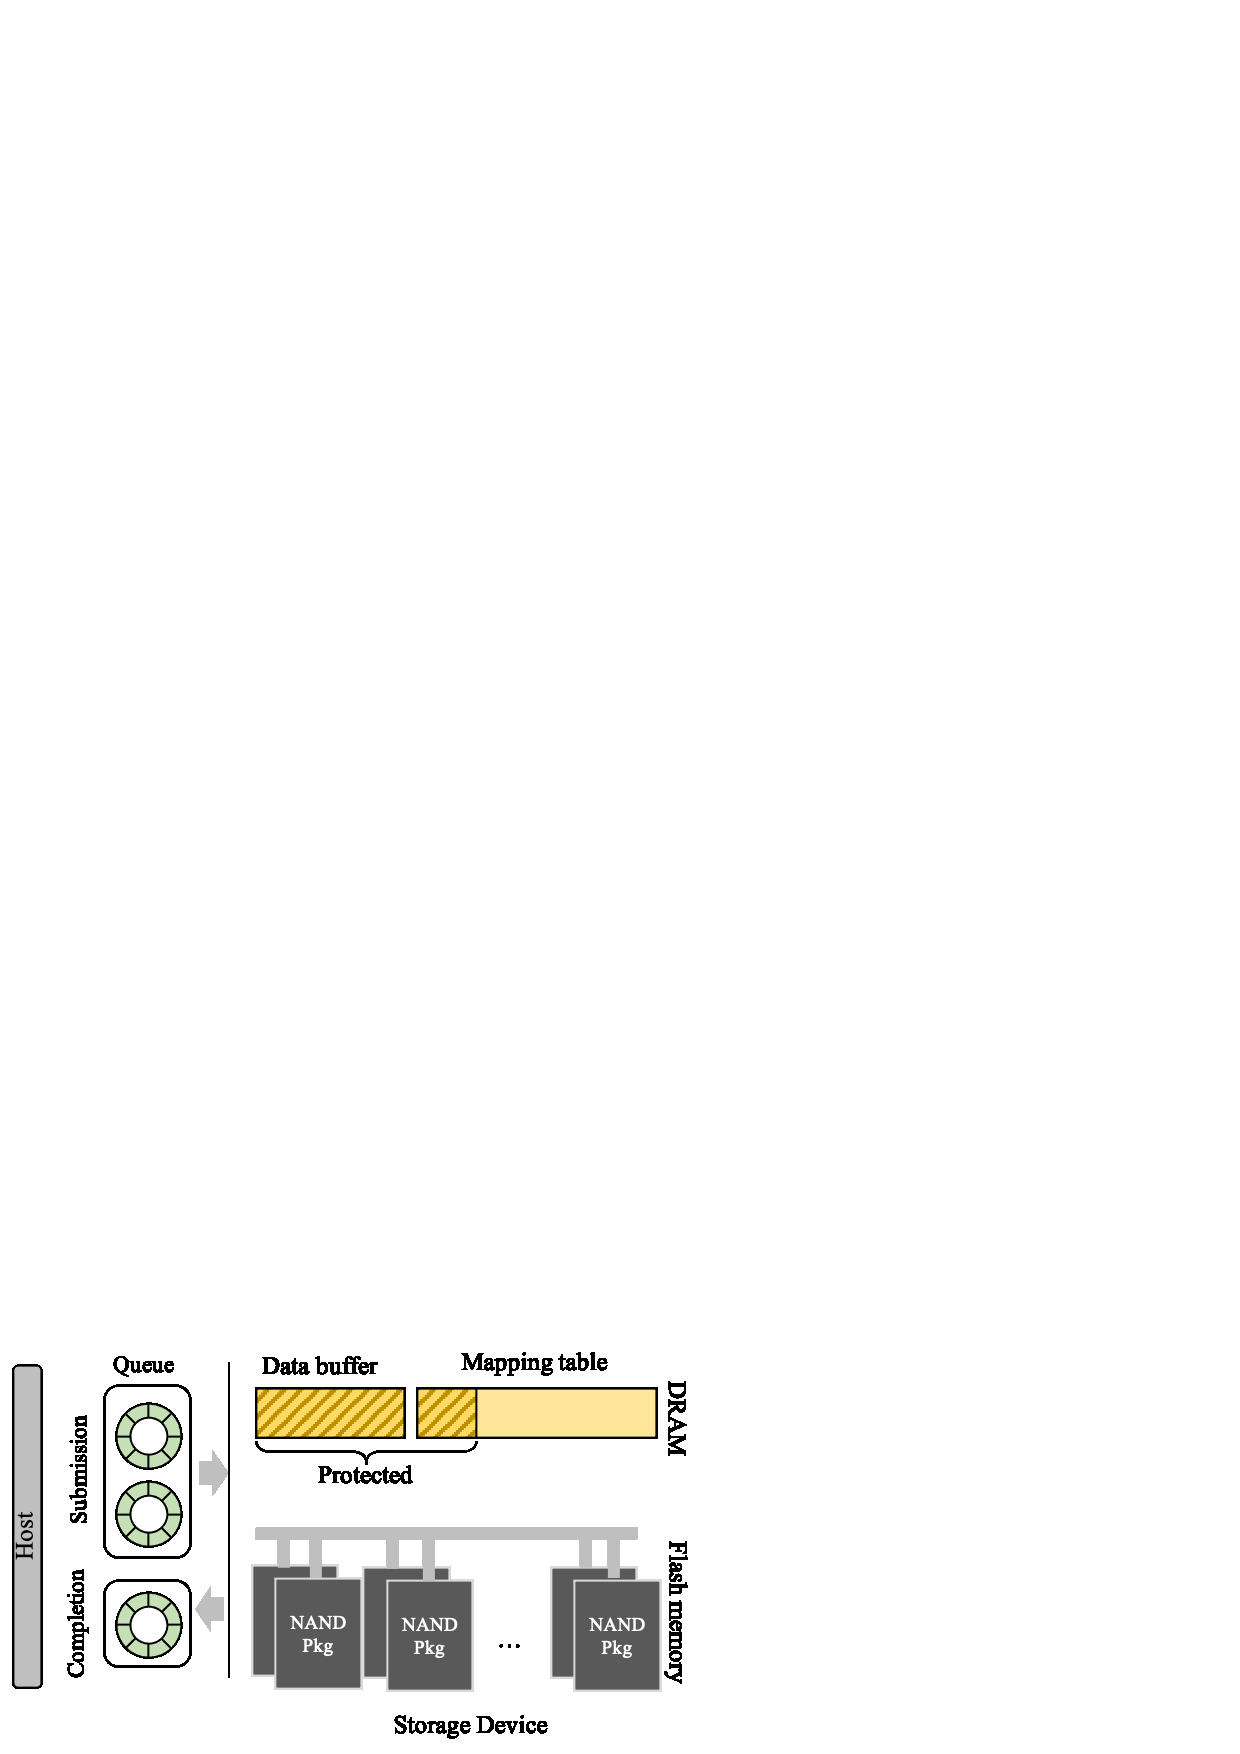
\includegraphics[width=0.4\textwidth]{figure/dawid_ssd_archi.png}
    \caption{\textbf{SSD architecture with Dawid buffer.}}
    \label{fig_spartan_archi}
\end{figure}

With this motivation, this paper presents an SSD-internal buffer architecture, called \ours{}, 
which operates under capacitance constraints. 
\ours{} essentially limits the number of dirty pages within buffer
to the level the maximum capacitance can protect.
If the number of dirty pages goes beyond the limit, they are flushed to flash memory. 
Note that the data maintained in buffer can be classified into two types: the actual user data and 
the metadata needed for their management in SSD (e.g., mapping table). 
In \ours{}, the capacitance constraint is applied only to the metadata, while protecting the user data entirely. 
This is because the storage suffers from serious performance degradation when the user data 
is not fully protected and should be entirely flushed upon a \texttt{FLUSH} command.

Based on this underlying architecture, \ours{} performs an I/O scheduling 
for the write requests within storage queue to reduce the write traffic
caused by the capacitance limitation. The scheduling algorithm aims to minimize the dirty page footprint 
of the internal buffer at a given time window. This behavior can reduce the frequency at which the number of dirty pages
exceeds the threshold and the modified pages are forced to flash memory. 
To this end, \ours{} prioritizes the write request with the least increase 
of the number of dirty pages in the mapping table.
With this policy, the write request of which the associated mapping page is already dirty 
has a top priority because it does not add the dirty page count. For other cases,  
% When the mapping page in clean state should be updated, 
\ours{} groups the write requests that modify the same mapping page 
and process them in batch in the order of group size. 
This policy enhances buffering and coalescing of the changes to the mapping table in the buffer, 
reducing a flush overhead significantly under capacitance constraints
compared to the FIFO (First-In First-Out) scheduling policy currently used in SSDs. 

To evaluate the effectiveness of \ours, we implement the proposed buffer design
in open-source SSD development framework. The performance evaluation with various workloads 
shows that \ours{} reduces the write traffic by up to 78\% and provides 25\% higher IOPS 
compared to the FIFO scheduling policy when only 10\% of the mapping table is protected. 
Compared to the full-protection architecture, \ours{} has has 20\% more writes and 
9\% of performance overhead, while reducing the required capacitance by 90\%. 

The remainder of this paper is organized as follows. In section 2, we briefly review the 
requirements and constraints for SSD with respect to reliability. Section 3 explains the 
design of SpartanSSD and Section 4 describes the implementation and performance evaluation results. 
Section 5 quantitatively analyzes the energy consumption of SSDs. Section 6 discusses our propoed design 
in relation to prior work, and Section 7 concludes. 


%define the cost for each data. the number of dirty pages increased 
% In contrast, the metadata is used only inside storage for device integrity or efficient indexing, 
% and thus it is more flexible to manage under capacitance constraints. 

%used for protecting device integrity and for accessing data 
% within storage. 

% In contrast, the metadata 
% user data 는 loss 가 발생하면 복구할 방법이 없는 반면, metadata 는 
% 사용자 데이터는 즉시 영구적으로 보호하는 것을 못한다면, 
% FLUSH command 처리에 따른 심각한 성능저하 초래. 
% host 는 반드시 flush command 를 보내야 하고, 그시점에 모든 데이터를 flush. 

% 반면 metadata 는 SSD가 해당 데이터를 잘 접근하고 SSD 자체의 integrity 유지를 위해 필요한 정보로, 
% 어느 정도 성능과 persistence 간의 

% protects user data 
%the storage buffer may be partially unprotected in power loss. 


\iffalse
\begin{itemize}
    \item capacitor density vs. SSD density 
    \item partially protected SSD 
    \item minimize the number of dirty page: write-back or management 
    \item user data cannot be managed by SSD 
    \item mapping table 의 더티 페이지 수를 줄일 수 있도록. 
\end{itemize}


A paragraph of text goes here.  Lots of text.  Plenty of interesting
text. \\

More fascinating text. Features\endnote{Remember to use endnotes, not footnotes!} galore, plethora of promises.\\
\fi
% %\vspace{-20pt}
\section*{Abstract}
The growth in SSD capacity is reaching its limit 
due to the stunted growth of capacitors---electrical components that store charge 
to protect data for the volatile memory in case of power loss. 
While the SSD's capacity scaled from 256GB in 2011~\cite{samsung2011} to 30TB in 2018~\cite{anandtech18samsung} (100$\times$), 
the density of Aluminum and Tantalum electrolytic capacitors only by tenfold from 1960 to 2005~\cite{both2015modern}.
This slow scaling will eventually limit the amount of DRAM that can be used in an SSD,
and this, in turn, will also limit the storage capacity as the size of DRAM and aggregate flash capacity proportionally scale~\cite{samsung_ratio, ni2017hash}. 

\iffalse
Enterprise-class SSDs provide a persistent internal buffer using the capacitors. 
This PLP(Power-Loss Protection) mechanism reached a limit as the SSD density outpaces the scaling capability of the capacitors. 
% The SSD has increased significantly in density for the past decade. 
% With the growing popularity of data-intensive applications, the SSD density has increased rapidly in recent years.
%, expanding by 100× over the past ten years [1], [15].
% As an example, 
In 2011, a typical 2.5-inch SSD had 256GB capacity, but
%the world's first 2TB SSD was released in 2013~\cite{foremay2013}, but 
by 2018, a high-capacity SSD boasted a 30TB, expanding by 100× over the past ten years
~\cite{samsung2011, anandtech18samsung}. 
\begin{comment}
This remarkable growth of the device-capacity is thanks to the advanced scaling technologies 
such as nanoscale fabrication~\cite{busche2014design} and multi-layer stacking~\cite{9365809}. 
\end{comment}
% As an example, in 2011, a typical 2.5-inch SSD had 256GB capacity with 256MB of DRAM; by 2018, a high-capacity 2.5- inch SSD boasted a 30TB with 40GB of
% Unfortunately, not all components of the SSDs have kept up with the scaling rate.
However, the capacitor fails to proceed at the pace. 
\begin{comment}
Historically, storage devices 
have been equipped with a small size of volatile buffer in front of the persistent disk. 
By using them as a write buffer, they hide a long latency of the physical storage medium 
as well as mitigating an endurance limitation of the worn-out devices. 
However, the volatile buffer loses all data in the event of power crash. 
To prevent a data loss or corruption by this, enterprise-class SSDs
rely on the capacitors; it reserves energy to persist data in volatile buffer 
in the unforeseen event of a power crash. 
In addition, the adoption of capacitors enables an SSD to ignore the \texttt{FLUSH} command that explicitly requests all data in the volatile buffer to be made durable.
This property increases the buffering effect in SSD significantly, leading to both less write traffic and a shorter operation latency.
% To overcome this limitation without sacrificing performance, 
The reliance on capacitors, however, has reached its limit. 
\end{comment}
% the improvement in capacitance fails to keep up with the rapid growth of SSDs. 
%Al(aluminum) and Ta(tantalum)-electrolytic capacitors used in SSDs have increased in density through miniaturization by tenfold from 1960 to 2005 [4]. 
The capacitance density has also steadily improved, but
it is not as rapid as the SSD scaling speed. 
Al(aluminum) and Ta(tantalum)-electrolytic capacitors used in SSDs 
have increased in density by tenfold from 1960 to 2005~\cite{both2015modern}. 
This is approximately 50x slower than the SSD density increase rate.
Given that the internal buffer size increases in proportion to the storage capacity (typically 0.1\% of storage capacity~\cite{samsung_ratio, ni2017hash}),
the density gap between capacitance and memory technologies 
imposes an intrinsic limitation on the current architecture wherein 
the entire buffer is protected by capacitors. 
\fi

This paper presents a device-internal buffer architecture called \ours{} 
for the SSDs under capacitance constraints. 
% which operates under capacitance constraints.
% Fig.~\ref{fig_dawid_archi} shows the SSD architecture targeted in our study. 
\iffalse
\textcolor{blue}{
Historically, storage devices have been equipped with a small size of volatile buffer in front of the persistent disk. By using them as a read cache and a write buffer, they hide a long latency of the physical storage medium as well as mitigating an endurance limitation of the worn-out devices.
However, the volatile buffer loses all data in the event of power crash. 
To prevent a data loss or corruption by this, enterprise-class SSDs
rely on the capacitors; it reserves energy to persist data in volatile buffer 
in the unforeseen event of a power crash. 
In addition, the adoption of capacitors enables an SSD to ignore the \texttt{FLUSH} command that explicitly requests all data in the volatile buffer to be made durable.
This property increases the buffering effect in SSD significantly, leading to both less write traffic and a shorter operation latency.
% \EUNJI{Need to make this part shorter}
}
\fi
% To overcome this limitation without sacrificing performance, 
% The reliance on capacitors, however, has reached its limit. 
\ours{} achieves a persistent buffer with small size of capacitance by answering the following two questions. 
%(1) what not to protect under capacitance limitation and (2) how to reduce the overhead of ensuring persistence for unprotected data.
First question is \textit{what not to protect under capacitance constraints}. The device-internal buffer is used for (1) caching translation information (i.e., mapping index) and (2) buffering user writes. 
% The data maintained in the buffer can be classified into two types: the actual user data and 
% the metadata for SSD management (i.e, mapping table). 
\ours{} applies the capacitance constraints only to translation information, while protecting the user data entirely. The user data write is synchronous with the user request and unrecoverable upon a power outage. It hampers user experiences seriously when unprotected. On contrary, 
translation information is entirely managed by the firmware and provides room for compromise when SSDs suffer from capacitance restriction. \EUNJI{Furthermore, the main culprit demanding buffer space is translation information because a flat structured table is widely used for its indexing and has a large memory footprint.} 
Second question is thus \textit{how to reduce the cost of ensuring persistence for the translation updates}. When the buffer is partially protected, the number of dirty pages is limited to the maximum amount of data that the on-board capacitance can protect. If it goes beyond the limit, changes should be immediately flushed to the flash memory. \ours{} mitigates the negative impact of this behavior with a capacitance-contraint aware I/O scheduling.
%to meet the durability constraint for SSDs. XX mapping table XX flush 줄여보자.

% otherwise durability violated. 
% \EUNJI{
% 보호되지 못하는 데이터가 있을 때 버퍼를 어떻게 관리하면, 보호되지 못하는 데이터의 persistence 를 유지하기 위해 발생하는 비용을 적게 발생시킬 것인가? 에 대한 질문. }
% \EUNJI{제안하는 기법: 부분적으로 보호되는 맵핑 테이블의 동기화 오버헤드를 줄이기 위해, 해당 비용을 최소로 증가시키도록 I/O 스케줄링을 하는 것임.}

%\section{Design of \ours{} Buffer}
% \section{Least Increase of Dirtiness Scheduling}
A primary way of  reducing the superfluous writes caused by a capacitance limitation is to maintain the dirty memory footprint below a protected threshold as long as possible. When a dirty page overflow occurs, flushing is forced and write amplification increases.
% The \ours{} buffer aims at minimizing the dirty memory footprint of the mapping table at any point in time.
To this end, \ours{} aggregates and batches the requests whose mapping entry resides in the same page. \EUNJI{This policy reduces the dirty memory footprint of the mapping table at any point in time, amortizing the synchronization overhead across more requests. As such, \ours{} delivers less write traffic and higher IOPS than existing scheduling (e.g., FIFO) under capacitance constraints. \ours{} maintains two data structures: \textit{a zero-cost list} that holds the write requests whose mapping table page is in dirty state, and \textit{a max binary heap} that maintains the mapping table page indexes sorted by the number of associated write requests. 
% We term this policy Least Increase of Dirtiness (LID) scheduling.
When NAND flash becomes idle, \ours{} sends a request from the (1) zero-cost list first and if it is empty, (2) from the max binary heap. 
}  
\iffalse
In this regard, the \ours{} buffer aims at minimizing the \textit{dirty memory footprint} of the mapping table at any point in time. To this end, \ours{} processes outstanding requests in the order that least increases the number of dirty pages in the mapping table. 
This scheme not only reduces the number of flushes for the mapping table partially protected but also increases the efficiency of flush operation by aggregating more translation updates into the smaller translation pages.
\fi

\iffalse
because (1) the data write is synchronous with the user request and (2) the user data takes up a relatively 
small footprint in the buffer. 
\fi
% This is because the storage suffers from serious performance degradation when the user data 
% is not fully protected and should be entirely flushed upon a \texttt{FLUSH} command.
% }
% \textcolor{brown}{
% \ours{} essentially limits the number of dirty pages within buffer
% to the level the maximum capacitance can protect.
% If the number of dirty pages goes beyond the limit, changes are flushed to the flash memory. 
% }
% \EUNJI{For this architecture, the problem boils down to how to reduce the write traffic to persist the mapping table to flash memory under capacitance constraints.
% \iffalse
Reducing the synchronization overhead of the mapping table is a well-known problem and has been extensively studied for a past decade~\cite{jiang2011s, kim2017shrd}. 
However, they mostly focus on the SSDs without PLP, which have different properties to the PLP-SSDs with capacitance constraints. 

\EUNJI{\ours{} is built upon the current trend of increasing queue depth of the storage interfaces. SATA and SAS support a single queue with 32 and 245 commands, but NVMe has 
up to 65,535 queues with as many as 65,536 commands per queue. 
This extension allows SSDs to further optimize the internal activities by taking advantage of the outstanding request information.
}

We implement \ours{} in \texttt{FEMU}, an open-source SSD development framework~\cite{li2018case}. Fig. XX shows that \ours{} reduces the write traffic by up to 78\% and provides 25\% higher IOPS 
compared to the FIFO scheduling when only 10\% of the mapping table is protected. 
Compared to the full-protection architecture, \ours{} has has 20\% more writes and 
9\% of performance overhead, while reducing the required capacitance by 90\%. 
Fig.XX shows 
\iffalse
To evaluate the effectiveness of \ours, we implement the proposed buffer design
in \texttt{FEMU}, which is an open-source SSD development framework~\cite{li2018case}. The performance evaluation with various workloads 
shows that \ours{} reduces the write traffic by up to 78\% and provides 25\% higher IOPS 
compared to the FIFO scheduling scheme when only 10\% of the mapping table is protected. 
Compared to the full-protection architecture, \ours{} has has 20\% more writes and 
9\% of performance overhead, while reducing the required capacitance by 90\%. 
\fi

\begin{figure}[t]
    \centering{}
    \includegraphics[width=0.20\textwidth]{shn-graph/rand-wt.eps}
    \includegraphics[width=0.20\textwidth]{shn-graph/rand-iops.eps}
    %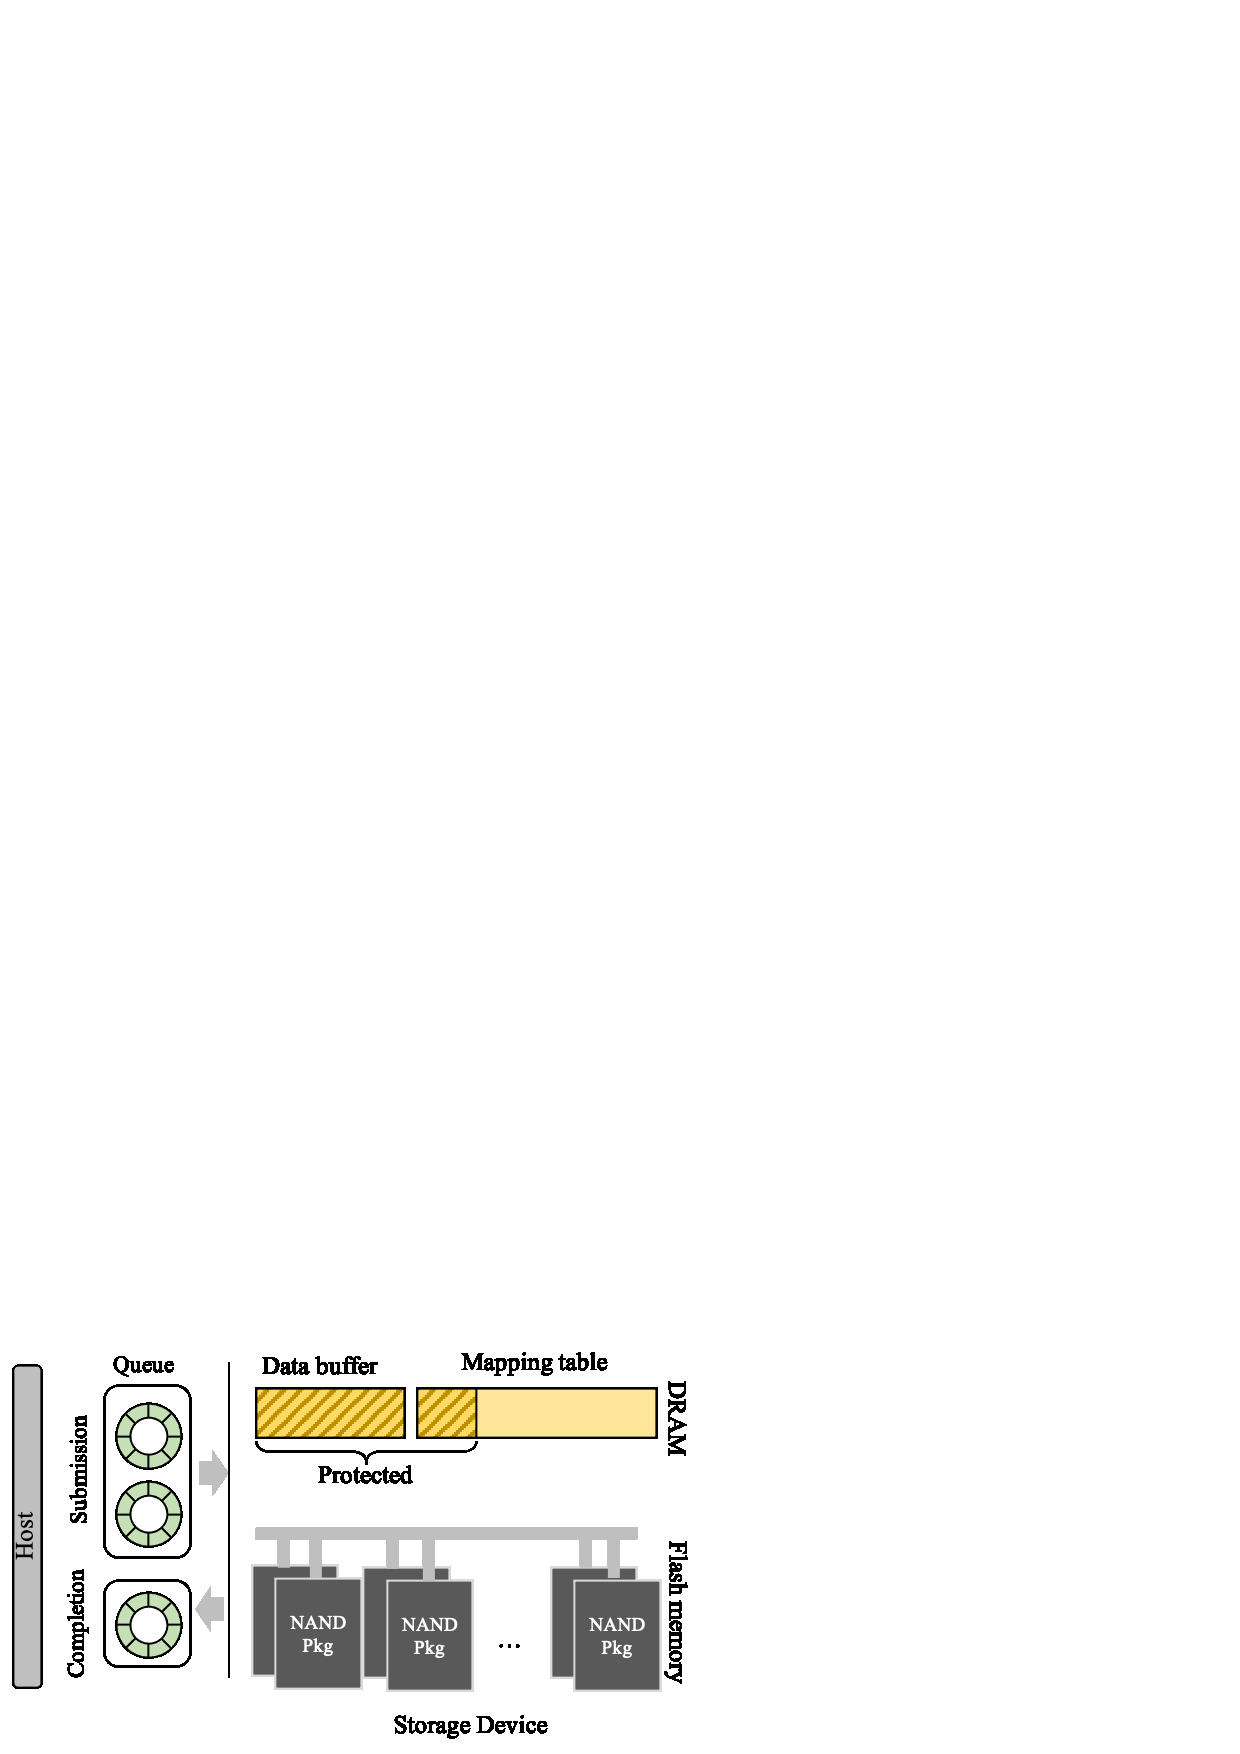
\includegraphics[width=0.4\textwidth]{figure/dawid_ssd_archi.png}
    \caption{\textbf{Write Traffic and IOPS (FIO-RAND).}}
    \label{fig_dawid_archi}
\end{figure}

\begin{figure}[t]
    \centering{}
    \includegraphics[width=0.20\textwidth]{shn-graph/jesd-wt.eps}
    \includegraphics[width=0.20\textwidth]{shn-graph/jesd-iops.eps}
    %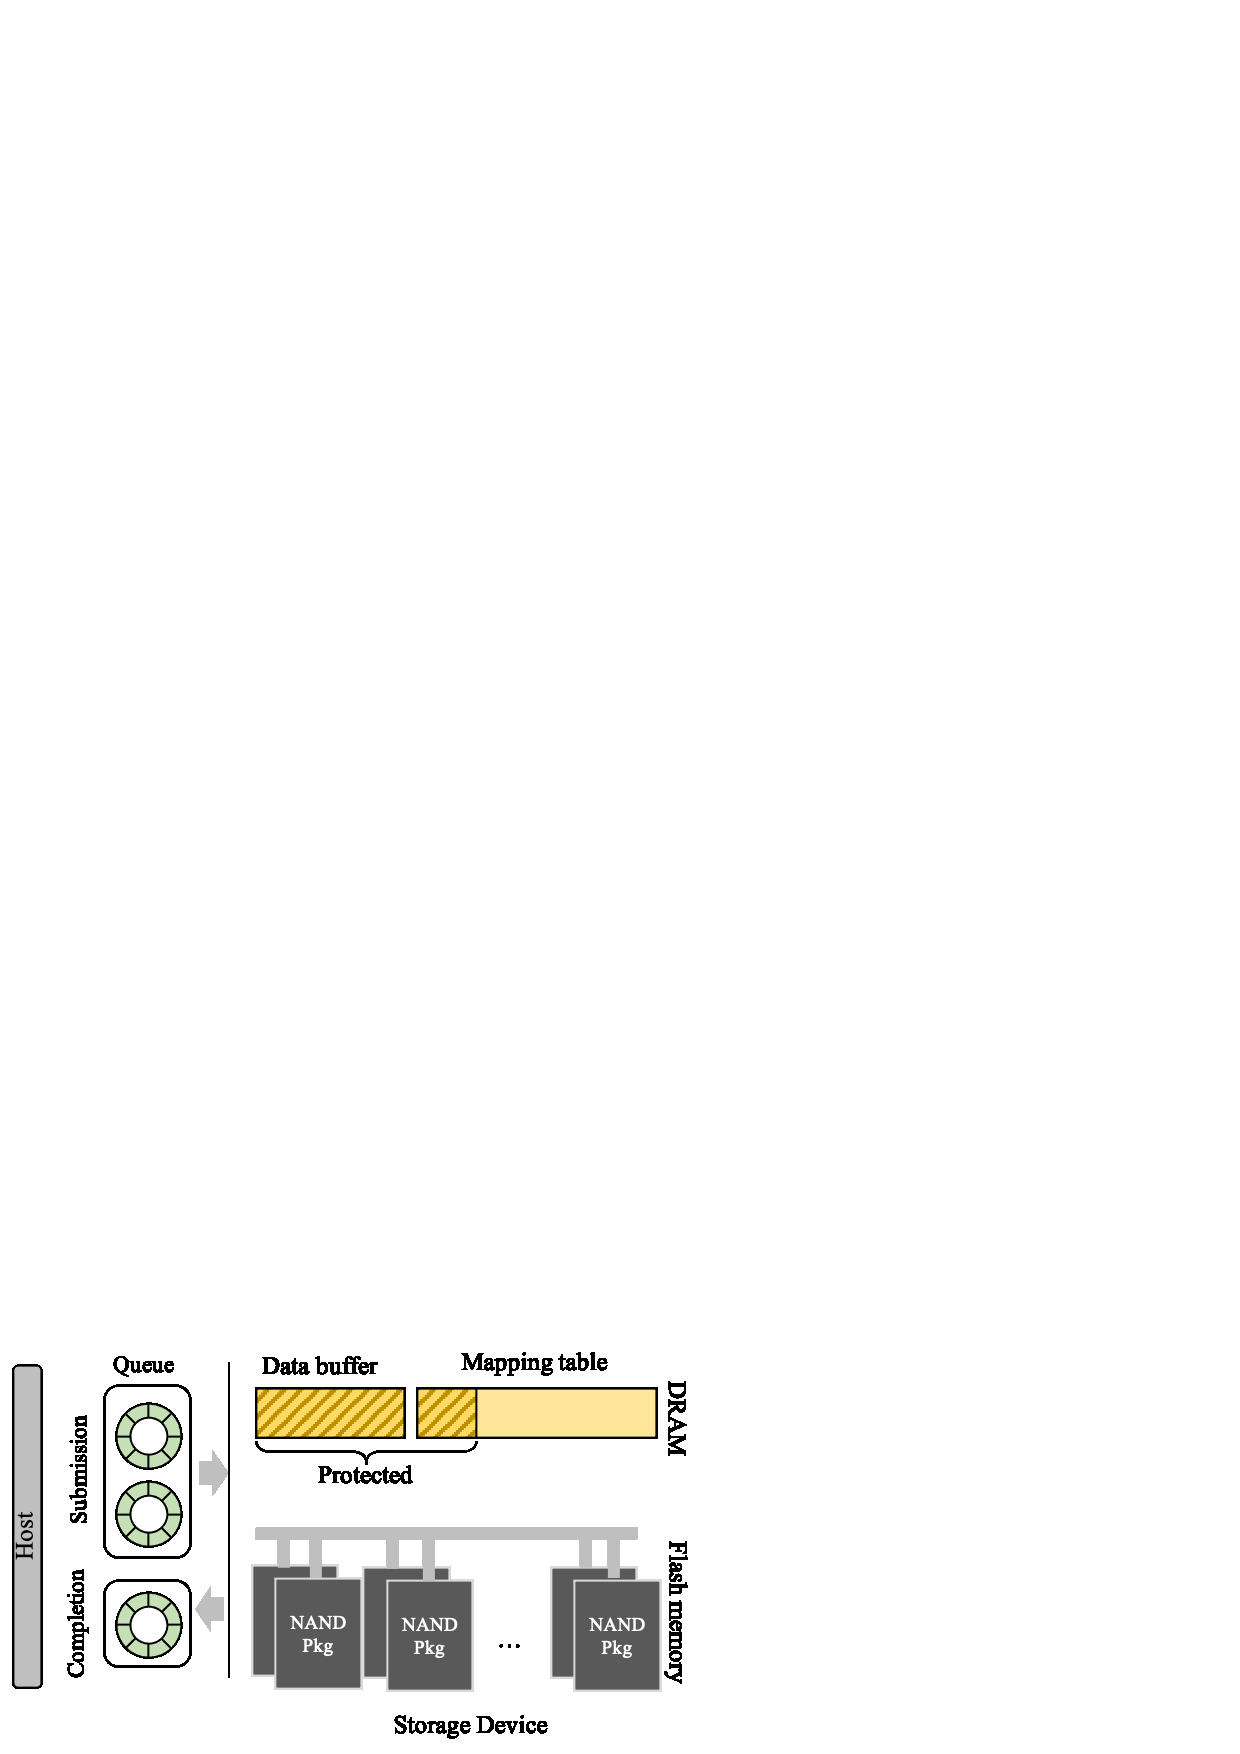
\includegraphics[width=0.4\textwidth]{figure/dawid_ssd_archi.png}
    \caption{\textbf{Write Traffic and IOPS (FIO-JESD) .}}
    \label{fig_dawid_archi}
\end{figure}

% \begin{figure}[t]
%     \centering{}
%     \includegraphics[width=0.5\textwidth]{figure/iops_write_traffic.png}
%     %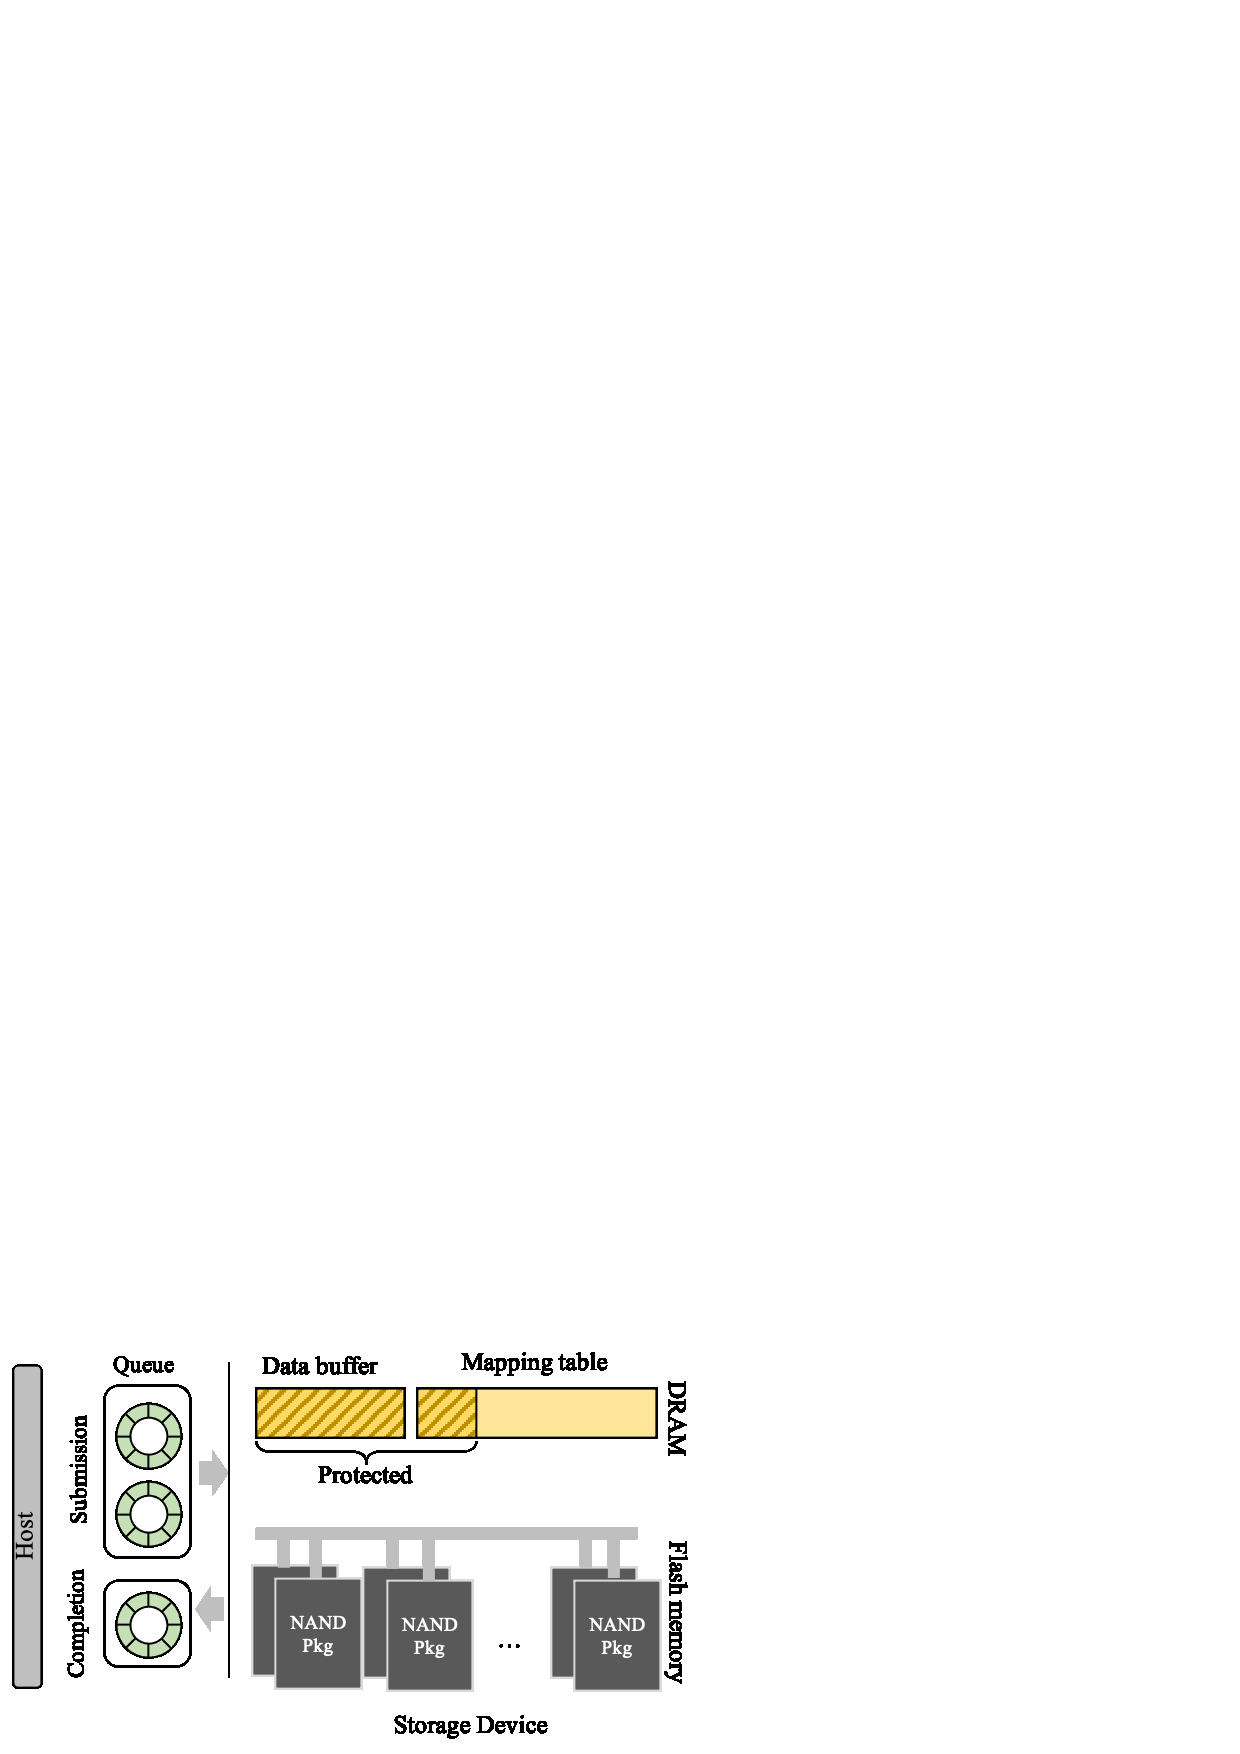
\includegraphics[width=0.4\textwidth]{figure/dawid_ssd_archi.png}
%     \caption{\textbf{IOPS and Write Traffic.}}
%     \label{fig_dawid_archi}
% \end{figure}

\input{02_related_work_short}
%\begin{figure*}[t!]
\begin{figure*}
    \centering{}
    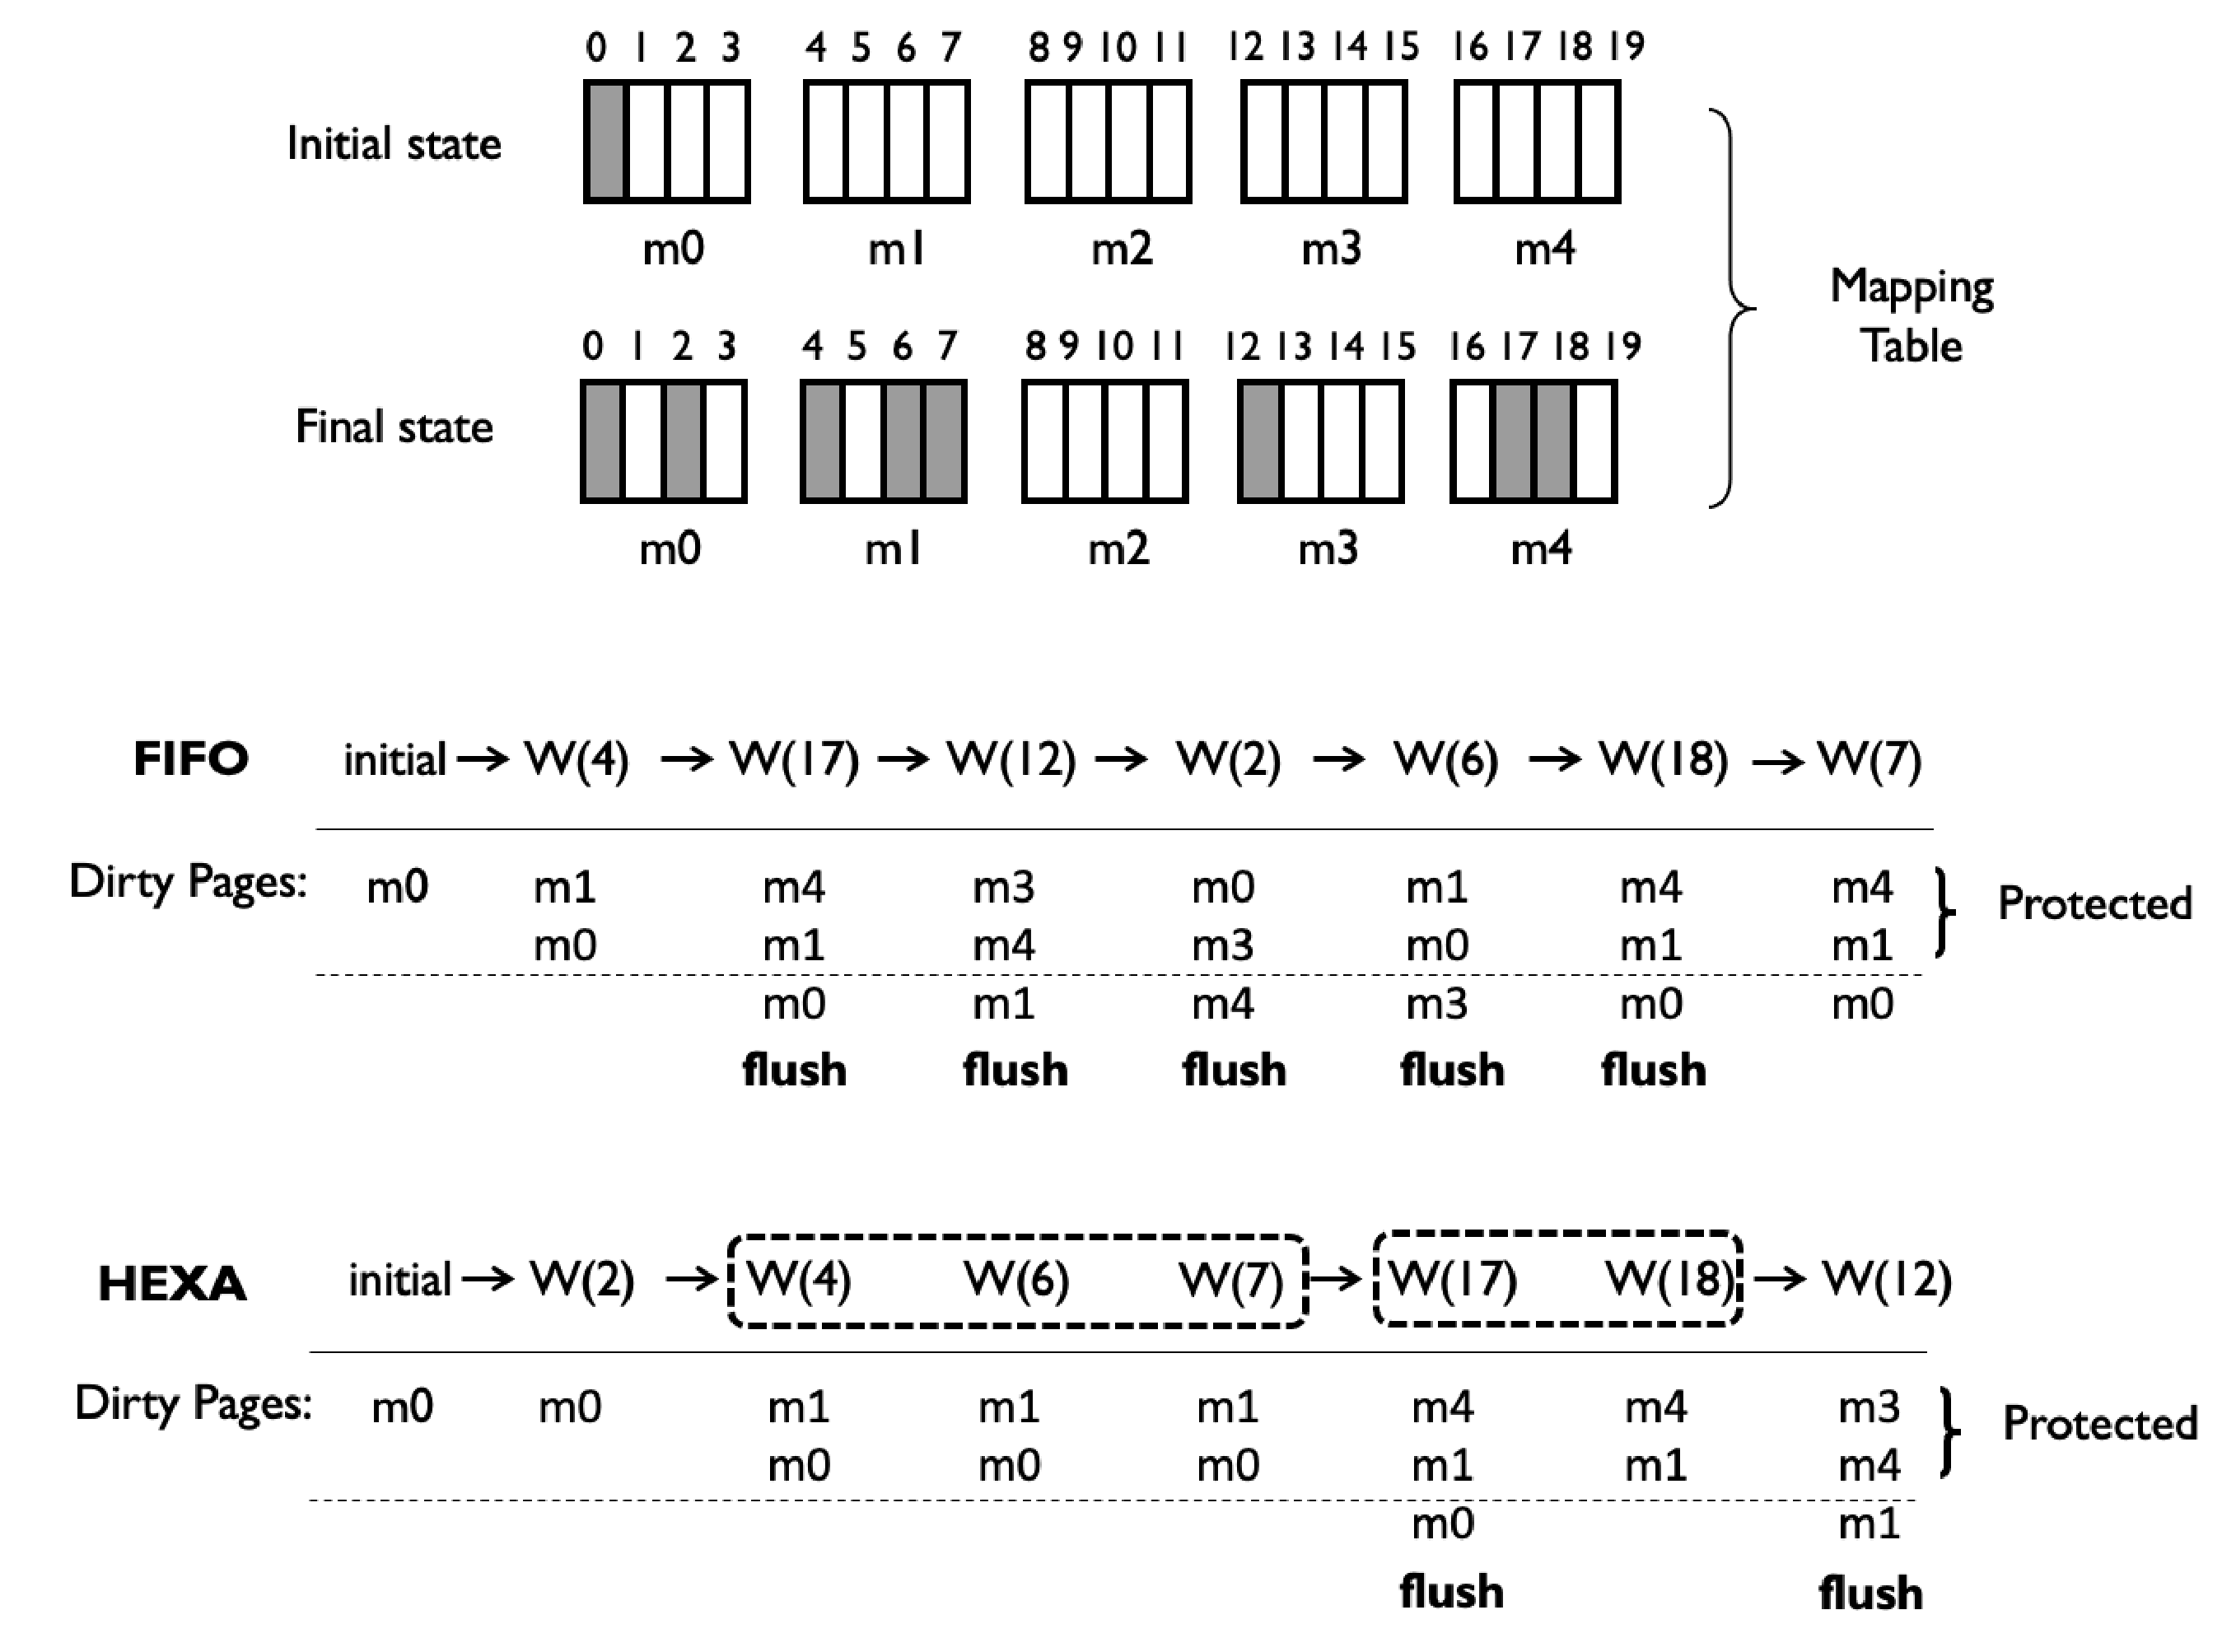
\includegraphics[width=0.8\textwidth]{figure/dawid_algo.eps}
    \caption{\textbf{Dawid Buffer Overview.}}
    \label{fig:dawid_buff_overview}
\end{figure*}

\section{Design}
This section describes the design and implementation of \ours{} buffer in detail. 
\S~\ref{subsec:overview} overviews the overall architecture of the in-storage buffer under capacitance constraints, and \S~\ref{subsec:lind_sched} presents the I/O scheduling algorithm
to reduce the write traffic in \ours{}.

\subsection{Overview}
\label{subsec:overview}
To satisfy a high demand for storage capacity in modern applications,
the SSDs have become highly scalable with advances in density-increasing techniques. 
The state-of-the-art SSDs provide tens of TBs capacity and this trend is expected 
to continue in the future.
The problem is that the capacitors, an integral component used in SSDs to protect the buffer data
in power outage, is unable to keep up with the significant density increase speed of NAND flash memory. 
The SSD-internal buffer is typically 0.1\% of the storage capacity in size.
To protect the entire buffer of SSD, the capacitors 
should have been improved at the same pace with SSD in density; 
its density has enhanced only at one-fifth speed of SSD density improvement. 
% This density gap between capacitors and memory technologies
% indicates that 
With this density gap, the PLP with full protection is no longer feasible in SSDs; 
it not only severely limits the form factor of SSDs requiring deployment of a large number of capacitors but also significantly increases the manufacturing cost of SSDs. 

\ours{} is designed to efficiently maintain the in-storage buffer under capacitance limitations. 
Table~\ref{tab:ssd_buff_comp} shows the breakdown of the in-storage buffer usage for each component
for 512GB SSD that has an architecture shown in Table~\ref{tab:ssd_config}. 
The user data buffer is employed to fully exploit the underlying flash parallelism.
Hence, it is typically twice the size of all pages that can be programmed in parallel, 
which is 4MB in this setting, while it may vary depending on the design choice. 
The mapping table that translates LPN(logical page number) to PPN(physical page number) 
accounts for 512MB, which corresponds to 97\% of the buffer size. 
Other metadata including mapping table directory uses a total of 10.5MB buffer. 

To overcome capacitance constraints for SSD, \ours{} sacrifices on some durability of mapping table, 
% by only protecting a portion of it, 
while protecting the user data and the metadata other than mapping table with capacitors. 
The user data persistence should be synchronously guaranteed with the host request
to conserve the properties of existing SSDs with PLP. 
For this reason, making a compromise on it can lead to a serious performance penalty in SSD.
On contrary, the requirements for the mapping table update are less stringent;
it does not have to be immediate upon a host request because the address translation is 
necessary only when the associated data is actually programmed to the flash memory. 
This nature allows a room for reasonable trade-off between capacitance and performance,
by effectively maintaining the persisting overhead of mapping table under capacitance constraint. 
Other metadata updates are also asynchronous with the host request, but
they use only a marginal space of the buffer; sophisticating their management mechanism 
for further capacitance saving is cost-ineffective. 

% because the PPN of data is determined when it is flushed to the flash memory. 
% The LPB to PPN translation is required when the data is in flash memory. 
% it can be restored on the reboot. 

% 요청된 데이터를 찾기 위해 사용. 
% 데이터는 보호되고 있는데 인덱스는 잃어버림. 
% ==> 추후 recovery 할 때 반영해주면 됨. 데이터를 쓰면서 업데이트 하거나 '
% ==> 이미 데이터가 플래시에 쓰여져 있다면? 걔는 보호를 해줘야 함. 
% ==> 대신 small write 임. 버퍼링 효과를 늘리면 footprint 를 줄일 수 있음. 

\iffalse
If an SSD has 8 channels and 4 ways per channel with 8KB page size, about 128KB of memory (twicethe  size  of  all  pages  that  can  be  written  in  parallel)  are  usedfor data buffering. This, however, only accounts for 0.02% ofthe volatile DRAM.
maximize the high degree of parallism in SSDs 
during the operation of flash memories 
\fi

% the end of full protection based SSD design 
%The capacitance faces scaling limit 

% mapping table 이 상당히 큰 부분을 차지한다. 
% 사용자 버퍼는 통상 SSD의 병렬성을 활용할 수 있는 정도로만 있으면 된다고 했지만, 
% 최근 다양한 이유로 증가하고 있음. 

\subsection{Least Increase of Dirtiness Scheduling}
\label{subsec:lind_sched}
\ours{} partially protects the mapping table with limited capacitance. 
When the dirty pages of mapping table become more than the maximum number of protected pages, 
\ours{} flushes them to flash memory based on the LRU (Least-recently Used) algorithm. 
Because this flush operation does not arise with SSD using PLP, mitigating the effect of this overhead 
is a key strategy to achieving high performance under capacitance constraints. 
To this end, \ours{} presents a cost-effective scheduling scheme for the in-storage buffer, called LIDF (Least Increase of Dirtiness First). 
LIDF prefers to force the user data that increases the dirtiness of the mapping 
table the least to flash memory. This scheme reduces the dirty page footprint 
of the mapping table at a time window by enhancing the locality of updates. 
As a result, the frequency of flush operation for the mapping table can be 
largely reduced. 

Figure~\ref{fig:dawid_buff_overview} compares the flush overhead of FIFO and LIDF scheduling in \ours{} buffer. 
In this example, there are seven write requests 
in the device queue, sent from host in the following order: \texttt{W(4)}, \texttt{W(17)}, \texttt{W(12)}, \texttt{W(2)}, \texttt{W(6)}, \texttt{W(18)}, and \texttt{W(7)}.  
The mapping table has one dirty page (\texttt{m0}) 
at an initial state. We assume that 2 out of 5 pages of the mapping table are protected. 
FIFO writes the user data in the buffer to flash memory in arrival order. 
With this scheme, the mapping table would be randomly updated, generating a large number of dirty pages at a 
time window. 
Consequently, FIFO incurs a total of five flushes of the mapping table page during the write process. 


In contrast, LIDF calculates the write cost for each data
that indicates an increase in the number of dirty pages of the mapping table when it is flushed, and it processes the request with minimum cost first. 
In this example, the write request \texttt{W(2)} has a top 
priority because its associated mapping table page (\texttt{m0}) is already dirty, and thus it does not add the dirty pages of the mapping table. 
Next, the write requests \texttt{W(4)}, \texttt{W(6)}, and \texttt{W(7)} are processed. 
Because their address mapping entries are located in the same page of the mapping table, the cost of flushing them 
is reduced to one third. 
With this policy, LIDF can reduce the footprint of mapping table updates within time intervals, thereby delivering only two flushes of the mapping table for the same task. 
 
\subsection{Eviction Policy}
\begin{figure}[t!]
    \centering{}
	\subfloat[JESD] { 
    	\includegraphics[width=0.2\textwidth]{expr/hitMap/eps/JESD_FIFO.eps}
    	\includegraphics[width=0.2\textwidth]{expr/hitMap/eps/JESD_DAWID.eps}
	} \\
	\subfloat[OLTP]{ 
    	\includegraphics[width=0.2\textwidth]{expr/hitMap/eps/OLTP_FIFO.eps}
    	\includegraphics[width=0.2\textwidth]{expr/hitMap/eps/OLTP_DAWID.eps}
	} \\
	\subfloat[Linkbench]{ 
    	\includegraphics[width=0.2\textwidth]{expr/hitMap/eps/JESD_FIFO.eps}
    	\includegraphics[width=0.2\textwidth]{expr/hitMap/eps/JESD_FIFO.eps}
	} \\
    \caption{\textbf{Write hit ratio for the protected range in a mapping table.}}
    \label{fig_dawid_archi}
\end{figure}




\begin{figure*}[!t]
    \centering{}
	\subfloat[IOPS] { 
	    \includegraphics[width=0.3\textwidth]{expr/micro_rslt_220525/perf/perf_RAND.eps}
	    \includegraphics[width=0.3\textwidth]{expr/micro_rslt_220525/perf/perf_JESD.eps}
	    \includegraphics[width=0.3\textwidth]{expr/macro_rslt_220601/perf/perf_OLTP.eps}
	} \\
	\subfloat[Write Traffic (UD: User Data, MD: Mapping Data, GUD/GMD: GC for User/Mapping Data)] { 
	    \includegraphics[width=0.3\textwidth]{expr/micro_rslt_220601/waf/RAND.eps}
        \includegraphics[width=0.3\textwidth]{expr/micro_rslt_220601/waf/JESD.eps}
        \includegraphics[width=0.3\textwidth]{expr/macro_rslt_220601/waf/OLTP.eps}
	} 
    % \caption{\textbf{IOPS}:\textit{F and H denotes FIFO and HEXA.}}
    \caption{\textbf{IOPS and WAF.} From left: Random, JESD, and TPC-C.}
    \label{fig_perf_iops}
    \vspace{-15pt}
\end{figure*} 

\iffalse
\begin{figure*}[!t]
    \centering{}
	\subfloat[IOPS] { 
	    \includegraphics[width=0.3\textwidth]{expr/micro_rslt_220525/perf/perf_RAND.eps}
	    \includegraphics[width=0.3\textwidth]{expr/micro_rslt_220525/perf/perf_JESD.eps}
	    \includegraphics[width=0.3\textwidth]{expr/macro_rslt_220601/perf/perf_OLTP.eps}
	} \\
	\subfloat[Write Traffic] { 
	    \includegraphics[width=0.3\textwidth]{expr/micro_rslt_220525/wt/RAND.eps}
        \includegraphics[width=0.3\textwidth]{expr/micro_rslt_220525/wt/JESD.eps}
        \includegraphics[width=0.3\textwidth]{expr/macro_rslt_220601/waf/OLTP.eps}
	} 
    % \caption{\textbf{IOPS}:\textit{F and H denotes FIFO and HEXA.}}
    \caption{\textbf{IOPS and Write Traffic.}}
    \label{fig_perf_iops}
    \vspace{-15pt}
\end{figure*} 
\fi
\iffalse
\begin{figure*}[!t]
    \centering{}
	\subfloat[Random] { 
	    \includegraphics[width=0.3\textwidth]{expr/micro_rslt_220525/perf/perf_RAND.eps}
	} 
	\subfloat[JESD] { 
	    \includegraphics[width=0.3\textwidth]{expr/micro_rslt_220525/perf/perf_JESD.eps}
	}
	\subfloat[TPC-C] {
	    \includegraphics[width=0.3\textwidth]{expr/macro_rslt_220601/perf/perf_OLTP.eps}
	} \\
%     \subfloat[TPC-C] {
% 	    \includegraphics[width=0.3\textwidth]{expr/macro_rslt_220525/perf/perf_OLTP.eps}
% 	}
	\subfloat[Random] { 
	    \includegraphics[width=0.3\textwidth]{expr/micro_rslt_220525/wt/RAND.eps}
	} 
	\subfloat[JESD] { 
	    \includegraphics[width=0.3\textwidth]{expr/micro_rslt_220525/wt/JESD.eps}
	}
% 	\subfloat[TPC-C] { 
% 	    \includegraphics[width=0.3\textwidth]{expr/macro_rslt_220525/wt/OLTP.eps}
% 	}
	\subfloat[TPC-C] { 
	    \includegraphics[width=0.3\textwidth]{expr/macro_rslt_220601/waf/OLTP.eps}
	}
    % \caption{\textbf{IOPS}:\textit{F and H denotes FIFO and HEXA.}}
    \caption{\textbf{IOPS and Write Traffic.}}
    \label{fig_perf_iops}
    \vspace{-15pt}
\end{figure*} 
\fi

\iffalse
\begin{figure*}[!t]
    \centering{}
	\subfloat[Random] { 
	    \includegraphics[width=0.3\textwidth]{expr/micro_rslt_220525/wt/RAND.eps}
	} 
	\subfloat[JESD] { 
	    \includegraphics[width=0.3\textwidth]{expr/micro_rslt_220525/wt/JESD.eps}
	}
% 	\subfloat[TPC-C] { 
% 	    \includegraphics[width=0.3\textwidth]{expr/macro_rslt_220525/wt/OLTP.eps}
% 	}
	\subfloat[TPC-C] { 
	    \includegraphics[width=0.3\textwidth]{expr/macro_rslt_220601/waf/OLTP.eps}
	}
	\caption{\textbf{Write Traffic.} \textit{UD - User Data, MD - Mapping Data, GUD - GC Write for User Data, GMD - GC Write for Mapping Data.}}
    \label{fig_perf_wt}
\end{figure*} 
\fi



\section{Evaluation}
%We assume 1\% of the mapping table is protected via capacitors in a 64GB SSD. 
%The 64GB SSD is using DRAM and assumes that 1\% of the mapping table is
%protected. 
We perform the experiments on a machine with a 20-core Intel Xeon(R) Silver
4114 CPU running at 2.2GHz and 84GB memory. We run FEMU (QEMU-based SSD
emulator) configured to use 10 cores, 4GB DRAM for main memory, and 16GB DRAM
for SSD emulation. We use page-level mapping and caches all translation pages in DRAM. 
The NAND flash chips include 8 channels and 8 flash
LUNs per channel. The page size is 8KB and there are 256 per-block pages. The
read and write latency is set to 60 and 700$\mu$s,
respectively~\cite{cheong2018flash}. We use the greedy algorithm for
GC (Garbage-Collection) and mount an Ext4 file system on the device.
% , which selects the least utilized block as a victim for cleaning. 
% The Ext4 file system is mounted on the emulated SSD.  
%Other configuration uses default settings of FEMU 

% We measure the average IOPS and the write traffic varying the protected ratio of a mapping table from 1\% to 100\%. 
The performance evaluation is conducted using three workloads.
% The fio benchmark~\cite{fio-bench} generates the 4KB of random writes and the
The fio benchmark generates the 4KB of random writes and the
skewed read-write mixed workload that follows JESD219 using 4 threads. A
total of 64GB of data was written to the 4GB area. For the real workload, we use 
TPC-C~\cite{council1990tpc} on MySQL, an online transactional processing benchmark.
% , which is executed using a sysbench benchmark suite~\cite{sysbench}.
For TPC-C, we precondition an SSD so that 75\% of the capacity is filled with data
and perform 0.1 million write queries using 10 threads.
% The TPC-C preconditions an SSD with data writes for 300 seconds and generates  
% write quries for 180 seconds using 10 threads.
For the performance comparison, we implemented a FIFO-SSD that processes 
write requests in arrival order.  

Fig.\ref{fig_perf_iops} shows the IOPS and Write Amplification Factor (WAF) of
the FIFO-SSD and \ours{} (denoted with a prefix F and H, respectively) when varying
the protected ratio of a mapping table from 1\% to 100\%.  We study two
different sizes of write buffer, 64MB and 1GB, to investigate the effectiveness
of \ours{} with respect to the queue depth. 
\iffalse
랜덤 워크로드에서 Hexa-SSD의 성능 향상폭이 가장 큼. mapping table locality 가
낮아 protected ratio 가 낮으면 mapping table flush 로 인한 traffic 증가가 컸음.
\ours{}는 buffer 내의 request re-ordering 을 통해 mapping table flush overhead
를 거의 제거함.  이에 protected ratio 가 1\% 이고 WB가 1GB일 때, WAF를 기존 2.3
인 것을 1.5로 낮춤. 이에 따른 성능향상도 1.4x 가 됨. 
\fi
As the figure shows, the random workload improves the most with \ours{}.  This
workload has low spatial locality innately, and thus it benefits enormously
from the re-ordering of \ours{}, in particular, 
when the buffer size is large. As a result, \ours{} with 1GB buffer
lowers WAF from 2.3 to 1.5 and enhances IOPS by 42.7\% when the protection
ratio is 1\%. 

For JESD and TPC-C, the result shows the same general trends as for the random
workload, while the performance gain becomes smaller because they have more skewed
access patterns. \ours{} with 1GB write buffer improves IOPS by 10\% and 
5.6\%, respectively, and reduces write amplification by 11.3\% and 3\% on average for a 
protection ratio under 10\%. 
In particular, TPC-C achieves little improvement because 
%its workload has a strong spatial locality bias, and thus 
the mapping table-related write originally accounts for only 5\% of the total traffic. 
For this reason, TPC-C exhibits more sensitivity to the buffer size than the write
traffic and it performs better with a smaller buffer.  We suspect
this effect is due to the increased software complexity as the buffer size
becomes larger. This can have a great impact on the performance of 
highly skewed and latency-sensitive database workloads. 
%, but we cannot be sure.  

Another counter-intuitive result is that \ours{} has slightly lower IOPS than
FIFO-SSD when the protected ratio is equal or above 50\%. Our careful analysis
reveals that the reordering of \ours{} distorts the original write pattern
generated by the host, which increases the possibility that pages with
different lifetimes are stored in the same block. This subsequently increases
the number of page-copy operations during GC, amplifying the write traffic. 
This is the case even when the workload is synthetic
random as all host writes transferred through a file system have a locality. 
%Therefore, distortion of host write pattern through re-ordering causes
%degradation of GC performance. 
Although the target environment of this paper is a case where the protected
ratio is low, to improve the generality of \ours{}, we will study
the effect of \ours{} on GC performance in more detail in the future.
%the technique that can alleviate the above problem in the future.


%\begin{figure*}[t]
%    \centering{}
%	\subfloat[OLTP] { 
%	    \includegraphics[width=0.3\textwidth]{expr/macro_220517/perf/OLTP/perf_OLTP.eps}
%	} 
%	\subfloat[Write Traffic] { 
%	    \includegraphics[width=0.3\textwidth]{expr/macro_220517/wt/OLTP/perf_OLTP.eps}
%	} 
%    \caption{\textbf{OLTP}}
%\end{figure*} 



%\begin{figure*}[t]
%    \centering{}
%	\subfloat[Sequential] { 
%	    %\includegraphics[width=0.3\textwidth]{expr/macro_220517/perf/OLTP/perf_OLTP.eps}
%	    \includegraphics[width=0.3\textwidth]{expr/micro_220517/perf/SEQ/perf_SEQ.eps}
%	} 
%	\subfloat[Random] { 
%	    \includegraphics[width=0.3\textwidth]{expr/micro_220517/perf/RAND/perf_RAND.eps}
%	} 
%	\subfloat[JESD] { 
%	    \includegraphics[width=0.3\textwidth]{expr/micro_220517/perf/JESD/perf_JESD.eps}
%	}
%    \caption{\textbf{IOPS}}
%\end{figure*} 
%




%\section{Performance Evaluation}


\begin{figure}[t]
    \centering{}
    \includegraphics[width=0.4\textwidth]{expr/micro/sw.eps}
    \includegraphics[width=0.4\textwidth]{expr/micro/rw.eps}
    %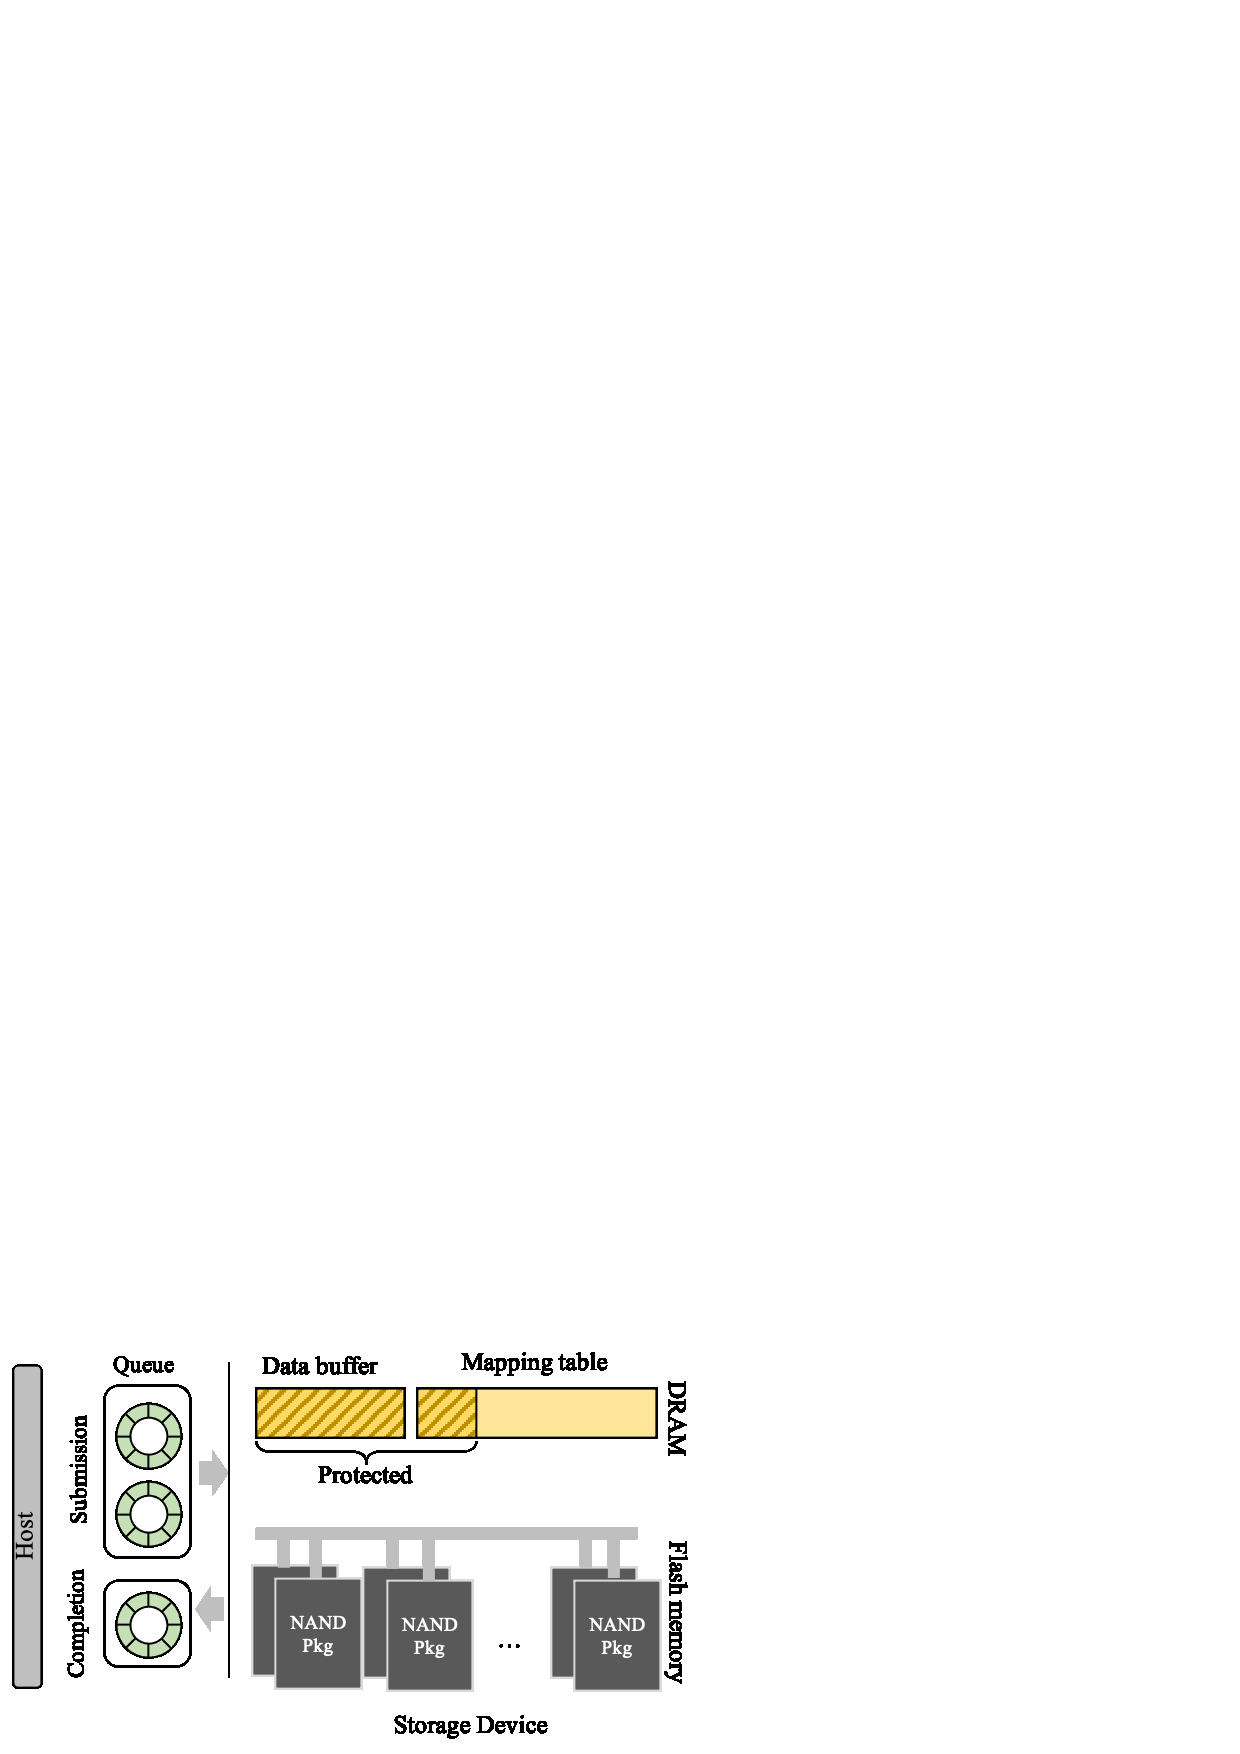
\includegraphics[width=0.4\textwidth]{figure/dawid_ssd_archi.png}
    \caption{\textbf{SSD architecture with Dawid buffer.}}
    \label{fig_spartan_archi}
\end{figure}


\subsection{Implementation}

\subsection{Performance results}

\section{Conclusion}
This paper presented a novel SSD design called \ours{}.
\ours{} protects a fraction of the storage-internal buffer to overcome capacitance constraints
in high-capacity SSDs. \ours{} maintains performance by reducing a dirty memory footprint 
of in-DRAM data through the cost-effective re-ordering, which underlies the increasing queue depth of the storage interfaces. 
%We implemented a \ours{}-SSD prototype in FEMU, an open-source SSD
%development framework. 
Performance evaluation with various workloads shows that \ours{} offers 
up to 42.7\% higher IOPS and 49\% less write traffic when the capacitance is highly limited.
% delivers only XX\%-XX\% performance slowdown when capacitance is reduced to 1\%, while conventional SSD using FIFO decreases performance by XX\%.

\iffalse
In this paper, we raised an issue about capacitance constraints in scalable
SSDs and presented a novel SSD design called \ours{} to overcome the
limitation.  \ours{}-SSD protects a part of the buffer, but reduces the dirty
memory footprint by exploiting the increasing queue depth of the storage
interfaces. We implemented a \ours{}-SSD prototype in FEMU, an open-source SSD
development framework. Performance evaluation using the prototype shows that \ours{}-SSD 
delivers only XX\%-XX\% performance slowdown when capacitance is reduced to 1\%, 
while conventional SSD using FIFO decreases performance by XX\%.
\fi

\iffalse
Hexa's design, implementation, and evaluation to
reduce performance overhead due to metadata flush in a situation where PLP is
partially supported on enterprise-class SSDs.  Our desing operates using only a
small amount of Capacitor's capacity compared to the previous one. It also
minimizes the impact of metadata by buffering requests using the scalability of
the write buffer.  Our evaluation results show that Hexa improves performance
in situations where requests are randomly generated.  In addition, JESD and
real-benchmark results comfirm that there are advantages in a real-world
environment.
\fi


\bibliographystyle{ieeetr}
{\small \bibliography{dawid_mascots}}


\end{document}
